\chapter{Time-memory tradeoff}

\paragraph{Summary}


\section{Time-memory tradeoff attack}

A brute-force attack on a block cipher would be to try out all the possible keys that could be used to encrypt certain known (or chosen) or unknown plaintext. The key which decrypts the ciphertext to give the known plaintext or most sensible plaintext (if it is unknown) is then the original key. Though very simple in theory, brute-force attacks require a very long time to break ciphers in practice. There is no storage required during this attack, but the time required to break the cipher is very long. Though modern computers have advanced tremendously in their computational speed over the last some years, design of new ciphers have incorporated longer key sizes to protect against brute-force attacks, thus not making brute-forcing any practical.

For example, in order to break a 32 bit key, we would need to carry out $2^{32}$ computations on available ciphertext. Using a 2GHz processor (which is quite common today for personal use), we can run $2^{31}$ clock cycles in one second. Since one encryption would take a fixed number of clock cycles, say a modest $2^2$ cycles, by simple calculation, we can have a brute-force attack on the cipher in $2^3$ seconds, or 8 seconds. As can be seen, this is a dismally weak key size. For a key size of 48 bits, the brute-force would take $2^{19}$ seconds which is 524288 seconds, or just more than 6 days. In modern ciphers, the key sizes starting from 128 bits in length are considered safe. AES uses a minimum key size of 128 bits, which can be extended to use 256 bits. 

Brute-force attacks are just one side of the coin. The other way of breaking a cipher in a known (or chosen) plaintext attack is to precompute ciphertexts corresponding to all the possible keys and to store the (key, ciphertext) pair in a table in memory. During the attack, the attacker just needs to do a table lookup for the available ciphertext, and get the corresponding key. Again, the concept is quite straightforward theoretically, but it also faces the same problem as brute-force attacks, but from a different perspective. A table lookup takes constant time, so practically the attack time is very less. But, the amount of precomputed data is tremendous and the attacker would need very large amount of memory to save this data for the attack phase. 

Let us take the weaker case of a 32 bit key, which is far from use in today's ciphers. For each of $2^{32}$ possible keys, we need to store 32 bits of key and 32 bits of ciphertext (assuming the plaintext is 32 bits, which could very well be more). This amounts to 64 bits or 8 bytes of data for every possible key. $2^{32}$ such entries would require $2^{32}$ * 8 bytes which is 32 gigabytes. For a random access memory, 32 GB is a high requirement. For higher key sizes, this requirement gets impossible to even think of.

The technique of time-memory tradeoff is a way between the above two extreme and practically difficult ideas. TMTO solves our problem by using memory in order to reduce the time taken for attack. As a result, with considerable precomputation, the attack time can be reduced and thus the computational resources required. It brings both the parameters, time and memory, within reachable domains. Before we go into more details of the working of time-memory tradeoff attacks on ciphers, we would take a simple example of a general application of such tradeoffs.

\paragraph{Simple example of time-memory tradeoff:} Consider the problem of finding the number of \textbf{1}'s in the binary expansion of a non-negative integer $x$. The simplest algorithm to solve this problem would over 32 operations, shift the integer rightwards by one bit (except for the first operation) and add the values of all the least significant bits. The sum would then be the \emph{result}. The pseudo-code for this is:

\begin{verbatim}
// ones_count(x)
t = 0
for i = 0 to len(x) - 1
    t = t + (x >> i) & 1
next i
return t
\end{verbatim}

Here, $>>$ denotes the right shift operation and \& denotes bitwise AND operation. This algorithm performs 32 operations (which is based on the number of times it loops) and has nearly no memory requirement. The other approach to solve this problem would be to store the required \emph{result} for each of the possible $2^{32}$ integers in memory. This way, just one memory lookup is required to find the result for $x$. While we need to have a memory of the order of $2^{32}$. One middle way between both these approaches would be to store the \textit{result} for all possible 8 bit numbers, rather than doing it for all 32 bit numbers. Then the memory required would be of the order of $2^{8}$. We break the 32 bit integer into four bytes, and add the stored \textit{result} for each of the bytes, by looking up in the table. If $y_1$, $y_2$, $y_3$ and $y_4$ are the four bytes, such that $y_4$ = ($x$ $\&$ $0$x$FF$), $y_3$ = ($(x >> 8)$ $\&$ $0$x$FF$), $y_2$ = ($(x >> 8)$ $\&$ $0$x$FF$) and $y_1$ = ($(x >> 8)$ $\&$ $0$x$FF$), and if p is the array which stores the \textit{result} for all possible bytes, then the \textit{result} for $x$ can simply be calculated by

\begin{verbatim}
t = p[y1] + p[y2] + p[y3] + p[y4]
\end{verbatim}

The number of operations in this case is 4, as the pre-computed table is looked up four times. This is just one way of realizing a middle way in between the extreme cases of time and memory. If the algorithm stores 4 bit values, with their corresponding \textit{result}, then the number of operations would be 8. Hence a optimum combination of memory and time can be selected depending on the resources at hand. 

\section{Birthday paradox}
\label{sec:bday-paradox}
Birthday paradox (or birthday problem or surprise, as it is also called), refers to the fact that in a room of 24 people, two people have the same date of birth with probability greater than one-half. While there are 365 different possible dates of birth, the birthday paradox looks surprising and non-intuituve at the first glance. But, the figure has been derived from probability theory and is proved. 

A generalized definition of the birthday paradox for can be formulated as follows: given $n$ random integers where each could have $m$ different possible values, the probability that two of them would have the same value is just more than \textbf{0.5} if,

\begin{equation*}
\begin{center}
\large{
$n$ = $\sqrt{\frac{\Pi}{\large{2}} \times m}$
}
\end{center}
\end{equation*}

If we replace $m$ by 365, then it can be easily checked that $n$ comes out to be 23.94, which can be taken as 24. The general birthday paradox is used in cryptography in determining the collisions in hash functions. Consider a hash function $H$ with output of $h$ bits. The total number of different outputs the function could produce is $2^{h}$. A collision is said to occur when the hash function produces the same output for two different inputs, i.e. $H(x_1)$ = $H(x_2)$ when $x_1$ $\neq$ $x_2$. Then, according to the birthday paradox, there are 50\% chances of finding a collision after the hash function hash produced outputs for $2^{n/2}$ random inputs.

A variant of the birthday paradox (\cite{GeneralizedAttack}) is especially more interesting to us, since it is directly used in TMTO attacks. If we consider two groups of people now, then just 17 people are required to be present in each group, so that two people from different groups share the same birthday. The answer is somewhat more complicated to calculate than the previous case. However, this case deals with the size of both the groups being the same. 

We are interested in the more general case dealing with two groups having different number of random elements, say $n_1$ and $n_2$. The groups contain integers, with both the groups having the same range $m$ for all the integers. Then, for there to be a common integer between the groups, the following relation must be satisfied,

\begin{equation*}
\begin{center}
\large{
$n_1 \times n_2}$ $\geq$ $m$
}
\end{center}
\end{equation*}

% Add the case of handbook statement, with or without replacements?
% also briefly how this paradox would be applied to the TMTO?

-------------
% what the simple birthday paradox is %

% generalize it in terms of n %

% introduce birthday attack, define scenario (then take hash as example) %

% what is the variant of birthday paradox %

% meet in the middle attack on DES by diffie hellman %
% a TMTO attack would always use variant of birthday attack %

% Question - How can the variant of the birthday problem be derived from the birthday problem?
% Question - Probability of one-half on 23, or is it one? root(pi * m / 2)
% Question - Is meet in the middle attack a TMTO attack? (I think NO!)
--------------


\section{Babbage-Golic attack}
Time-memory tradeoff attacks on stream ciphers are relatively new than those on block ciphers. The first TMTO attack on block ciphers was published by Hellman in 1980. In contrast, the first and the simplest TMTO attack on stream ciphers was published by Babbage \cite{babbage} and Golic \cite{golic}, independent of each other in 1995 and 1997 respectively. We would call this as the BG attack and explain it here. 

As discussed in section \ref{sec:psrg}, PRSG generates a long keystream using a short secret key, to which the bits of the plaintext are xor'ed giving the ciphertext bits. In this way, a stream cipher is produced. A simple model of the PRSG taken from \cite{babbage} is shown in figure \ref{fig:psrg-model}. The initial state of the PRSG is $S_0$, which is derived using the secret key and other initialization parameters. The consequent states are indicated by $S_i$. The right arrow represents the update function or the state transition function, while the downward arrow represents the output function of the PRSG.

\begin{figure}[h]
	\centering
	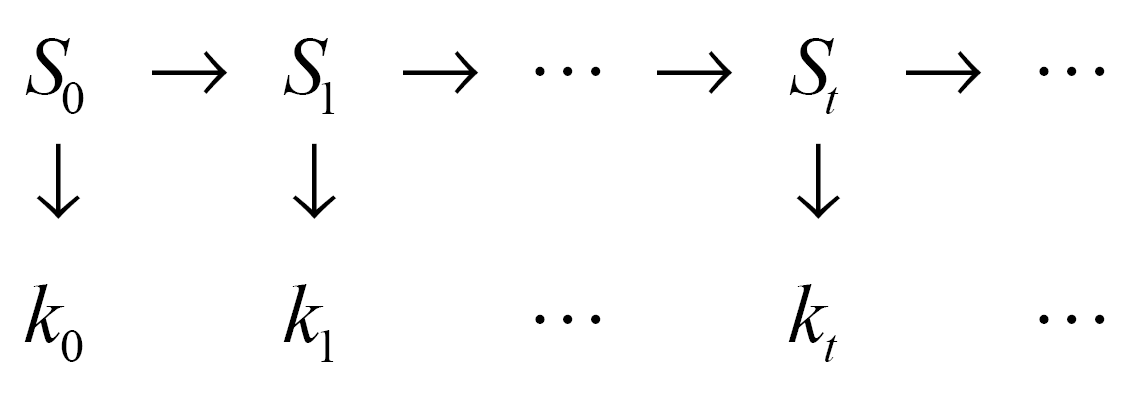
\includegraphics[width=3in]{./figures/prsgmodel.png}
	\caption{Model of pseudo-random sequence generator (PRSG)}	
	\label{fig:psrg-model}
\end{figure}

If the size of each state is $n$ bits, then the maximum number of different states would be $2^n$. As a result, we have $2^n$ different keystream bits, before the keystream starts repeating due to repeating states. The keystream bits are represented by $k_0$, $k_1$ $\ldots$, $k_{m-1}$, where $m$ = $2^{n} - 1$ (which excludes the trivial state containing all \textbf{0}'s). The goal of the attacker is to find at least one value of the internal state which occurs during the generation of the keystream. The attacker could then move the PRSG forward to generate more keystream (if the keystream is limited). The found internal state could also be used to run the PRSG backwards and find the initial state. From the initial state, finding the key is not a difficult task if the initialization algorithm and other parameters are known.\\

\textit{\textbf{Prefix of the output sequence of states.}} If the current state of the PRSG is $S_r$, then an infinite output sequence can be generated by clocking the PRSG from that state. The first $p$ bits of this output sequence is called the prefix of state $S_r$ and would be represented by the bits $k_r$, $k_{r+1}$ $\ldots$, $k_{r+p-1}$. Each of the $2^n$ possible states of the PRSG would have such output sequence and thus prefixes, which usually are unique to that particular state if $p$ is greater than or equal to $n$ \cite{}. If the size of the prefix is less than $n$, then there would be many states which could possibly generate this prefix. For example, if the size of the state is 48 bits and we consider prefixes of size 32 bits, then the total number of states which generate this prefix is about $2^{48} \times 2^{-32}$ = $2^{16}$. If the size of the prefixes is increased to 48 bits which is also the size of the state, then there is usually just one state generating the prefix. An advantage of this property is taken in the BG attack.\\

\textit{\textbf{The attack.}} We would have two phases in the attack just as in any TMTO attack. The first phase is the precomputation phase and the second phase is the attack phase. During the precomputation phase, the attacker would randomly select $n_1$ values out of the $2^n$ values the PRSG state could have. For each of these states, the prefix is computed, and the (prefix, state) pair stored in memory. The data structure that needs to be used for storing the pairs is a hash table. More details about hash tables are provided in section ??.

During the attack phase, the attacker is assumed to have access to some part of the initial keystream. In practice, the attacker would have access to the ciphertext bits. But, we assume that the attacker knows the plaintext bits before hand by some means, and thus the keystream is calculated in the following manner, $k_i$ = $p_i \oplus c_i$, as also mentioned in chapter \ref{chapter:intro}. The attacker then selects overlapping subsequences of size $n$ from the keystream, and tries to find a match in the hash table. The first subsequence would be $k_0$, $k_1$ $\ldots$, $k_{n-1}$ corresponding to state $S_0$, the second subsequence would be $k_1$, $k_2$ $\ldots$, $k_{n}$ corresponding to state $S_1$, and so on. If such a prefix exists in the memory, then the current state is determined from the matched (prefix, state) pair.\\

\textit{\textbf{Analysis of the attack.}} Let us assume that the attacker tries $n_2$ prefixes during the attack phase, before the first hit is observed. Then, we can apply the birthday paradox here, in order to find the approximate value of $n_2$. According to the variant of the birthday paradox, explained in section \ref{sec:bday-paradox}, we have the following condition:
\begin{equation*}
\begin{center}
\large{$n_1 \times n_2$ $\geq$ $2^n$}
\end{center}
\end{equation*}

Also, for sufficient number of prefixes to be available, the keystream should have a length of at least $(n_2 + n - 1)$ bits. In such a case, the attacker would have exactly $n_2$ prefixes of length $n$ each to search in the memory.


\section{Babbage-Golic attack on HiTag2}

\section{Variant of Babbage-Golic attack on HiTag2}

